\documentclass[a4paper,10pt]{article}
%A Few Useful Packages
\usepackage{marvosym}
\usepackage{fontspec,enumitem} 					%for loading fonts
\usepackage{xunicode,xltxtra,hyperref,parskip} 	%other packages for formatting
\usepackage[margin=2.5cm]{geometry}
\RequirePackage{color,graphicx}
\usepackage[usenames,dvipsnames]{xcolor}
\usepackage[big]{layaureo} 				%better formatting of the A4 page
% an alternative to Layaureo can be ** \usepackage{fullpage} **
\usepackage{array,xeCJK}
\usepackage{titlesec}					%custom \section
\setlist[itemize]{leftmargin=0pt}

%Setup hyperref package, and colours for links
\usepackage{hyperref}
\definecolor{linkcolour}{rgb}{0,0.2,0.6}
\hypersetup{colorlinks,breaklinks,urlcolor=linkcolour, linkcolor=linkcolour}

%FONTS
\defaultfontfeatures{Mapping=tex-text}
\newfontface\TitleFont{Noto Sans}
\setmainfont{Noto Sans}
\setsansfont{Noto Sans}
\setCJKmainfont{Source Han Sans TW}

\titleformat{\section}{\large\bfseries\TitleFont\raggedright}{}{0em}{}[\titlerule]
\titlespacing{\section}{0pt}{1em}{0.5em}

\setlength{\parindent}{0pt}
\newcommand{\leftcolumn}{0.6\textwidth}
\newcommand{\wideleftcolumn}{0.75\textwidth}
\newcolumntype{L}{>{\raggedright\arraybackslash}p{\leftcolumn}}
\newcolumntype{W}{>{\raggedright\arraybackslash}p{\wideleftcolumn}}
\newcommand{\rightcolumn}{\textwidth-\leftcolumn-1cm}
\newcommand{\narrowrightcolumn}{\textwidth-\wideleftcolumn-1cm}
\newcolumntype{R}{>{\raggedleft\arraybackslash}p{\rightcolumn}}
\newcolumntype{X}{>{\raggedleft\arraybackslash}p{\narrowrightcolumn}}
\newcommand{\tablespacer}{\multicolumn{2}{c}{}\\}
\newcommand{\entry}[1]{\textsf{#1}}
\newcommand{\md}{$\cdot$ }
\newenvironment{cvtable}{\begin{tabular}{WX}}{\end{tabular}}
\newenvironment{cvtable*}{\begin{tabular}{LR}}{\end{tabular}}


\begin{document}
\frenchspacing

% Title
\begin{center} 
  \Huge{
\includegraphics[height=1.3em,trim=0 10mm 0 -1cm]{shared/signature.png}}\par
  \normalsize {116 台北市文山區羅斯福路五段245號3樓之7}

  
\includegraphics[height=0.7em]{shared/mobile-alt.eps} +886~910-384-478 $\cdot$
  
\includegraphics[width=0.8em]{shared/envelope.eps} 1119han@gmail.com $\cdot$
  
\includegraphics[width=0.8em]{shared/github.eps}
  \href{https://github.com/RocketSH}{github.com/RocketSH}
\end{center}

\rule{15.2cm}{0.05em}

\vspace*{1em}
\begin{center}
  \large{應徵職位: 前端工程師}
\end{center}
\vspace*{1em}

\begin{center}
  \begin{minipage}{0.9\textwidth}
        2015年於寶成工業東莞分公司擔任戶外專業運動鞋\underline{開發產品報價管理師},
        具備專案管理、時程控管、跨部門溝通、數字分析專長;
        2017年起升任越南胡志明分公司報價團隊資深管理師,定期往返中國、法國、台灣執行品牌\underline{業務分析}與\underline{商業簡報}。2019年主動請調加入SAP導入專案
        ,除擔任\underline{內部講師}也負責\textbf{數據轉換邏輯、排除錯誤、系統
          測試}。

        \vspace*{1em}
        2020年初利用3個月於Astro Camp學習\textbf{HTML, CSS, Bootstrap, Ruby on
          Rails, JavaScript, Git版本控制},並自學\textbf{PostgreSQL資料庫操作, React框架}。
  \end{minipage}
\end{center}

\vspace*{1em}
\begin{center}
  \large{相關作品}
\end{center}
\hspace*{1em}\entry{個人網站}

\includegraphics[width=0.8em]{shared/globe-asia.eps}
\href{https://rocketgirl.io/}{rocketgirl.io}

\hspace*{1.5em}{前端:ReactJS, HTML, CSS}

\hspace*{1.5em}{後端:GatsbyJS}

\begin{minipage}{0.5\textwidth}
  \hspace*{1em}\entry{電子報平台}
  
\includegraphics[width=1em]{shared/mail.png}
  \href{https://www.goodbyt.es/}{goodbyt.es}

  \vspace*{.5em}
  \hspace*{1.5em}{[前端] HTML, CSS, Bootstrap, SortableJS,}
  \hspace*{1.5em}{Stimulus, AJAX}
  
  \vspace*{.5em}
  \hspace*{1.5em}{[Ruby Gem] devise, Nokogiri, Carrierwave}
  \hspace*{1.5em}{+AWS S3}

  \vspace*{.5em}
  \hspace*{1.5em}{[後端] Ruby on Rails} 

  \vspace*{.5em}
  \hspace*{1.5em}{[資料庫] PostgreSQL} 

  \vspace*{.5em}
  \hspace*{1.5em}{[寄信服務商] Mailgun} 
  \vspace*{1em}

\end{minipage}%
\begin{minipage}{0.5\textwidth}
\vspace*{.8em}
\begin{center}
  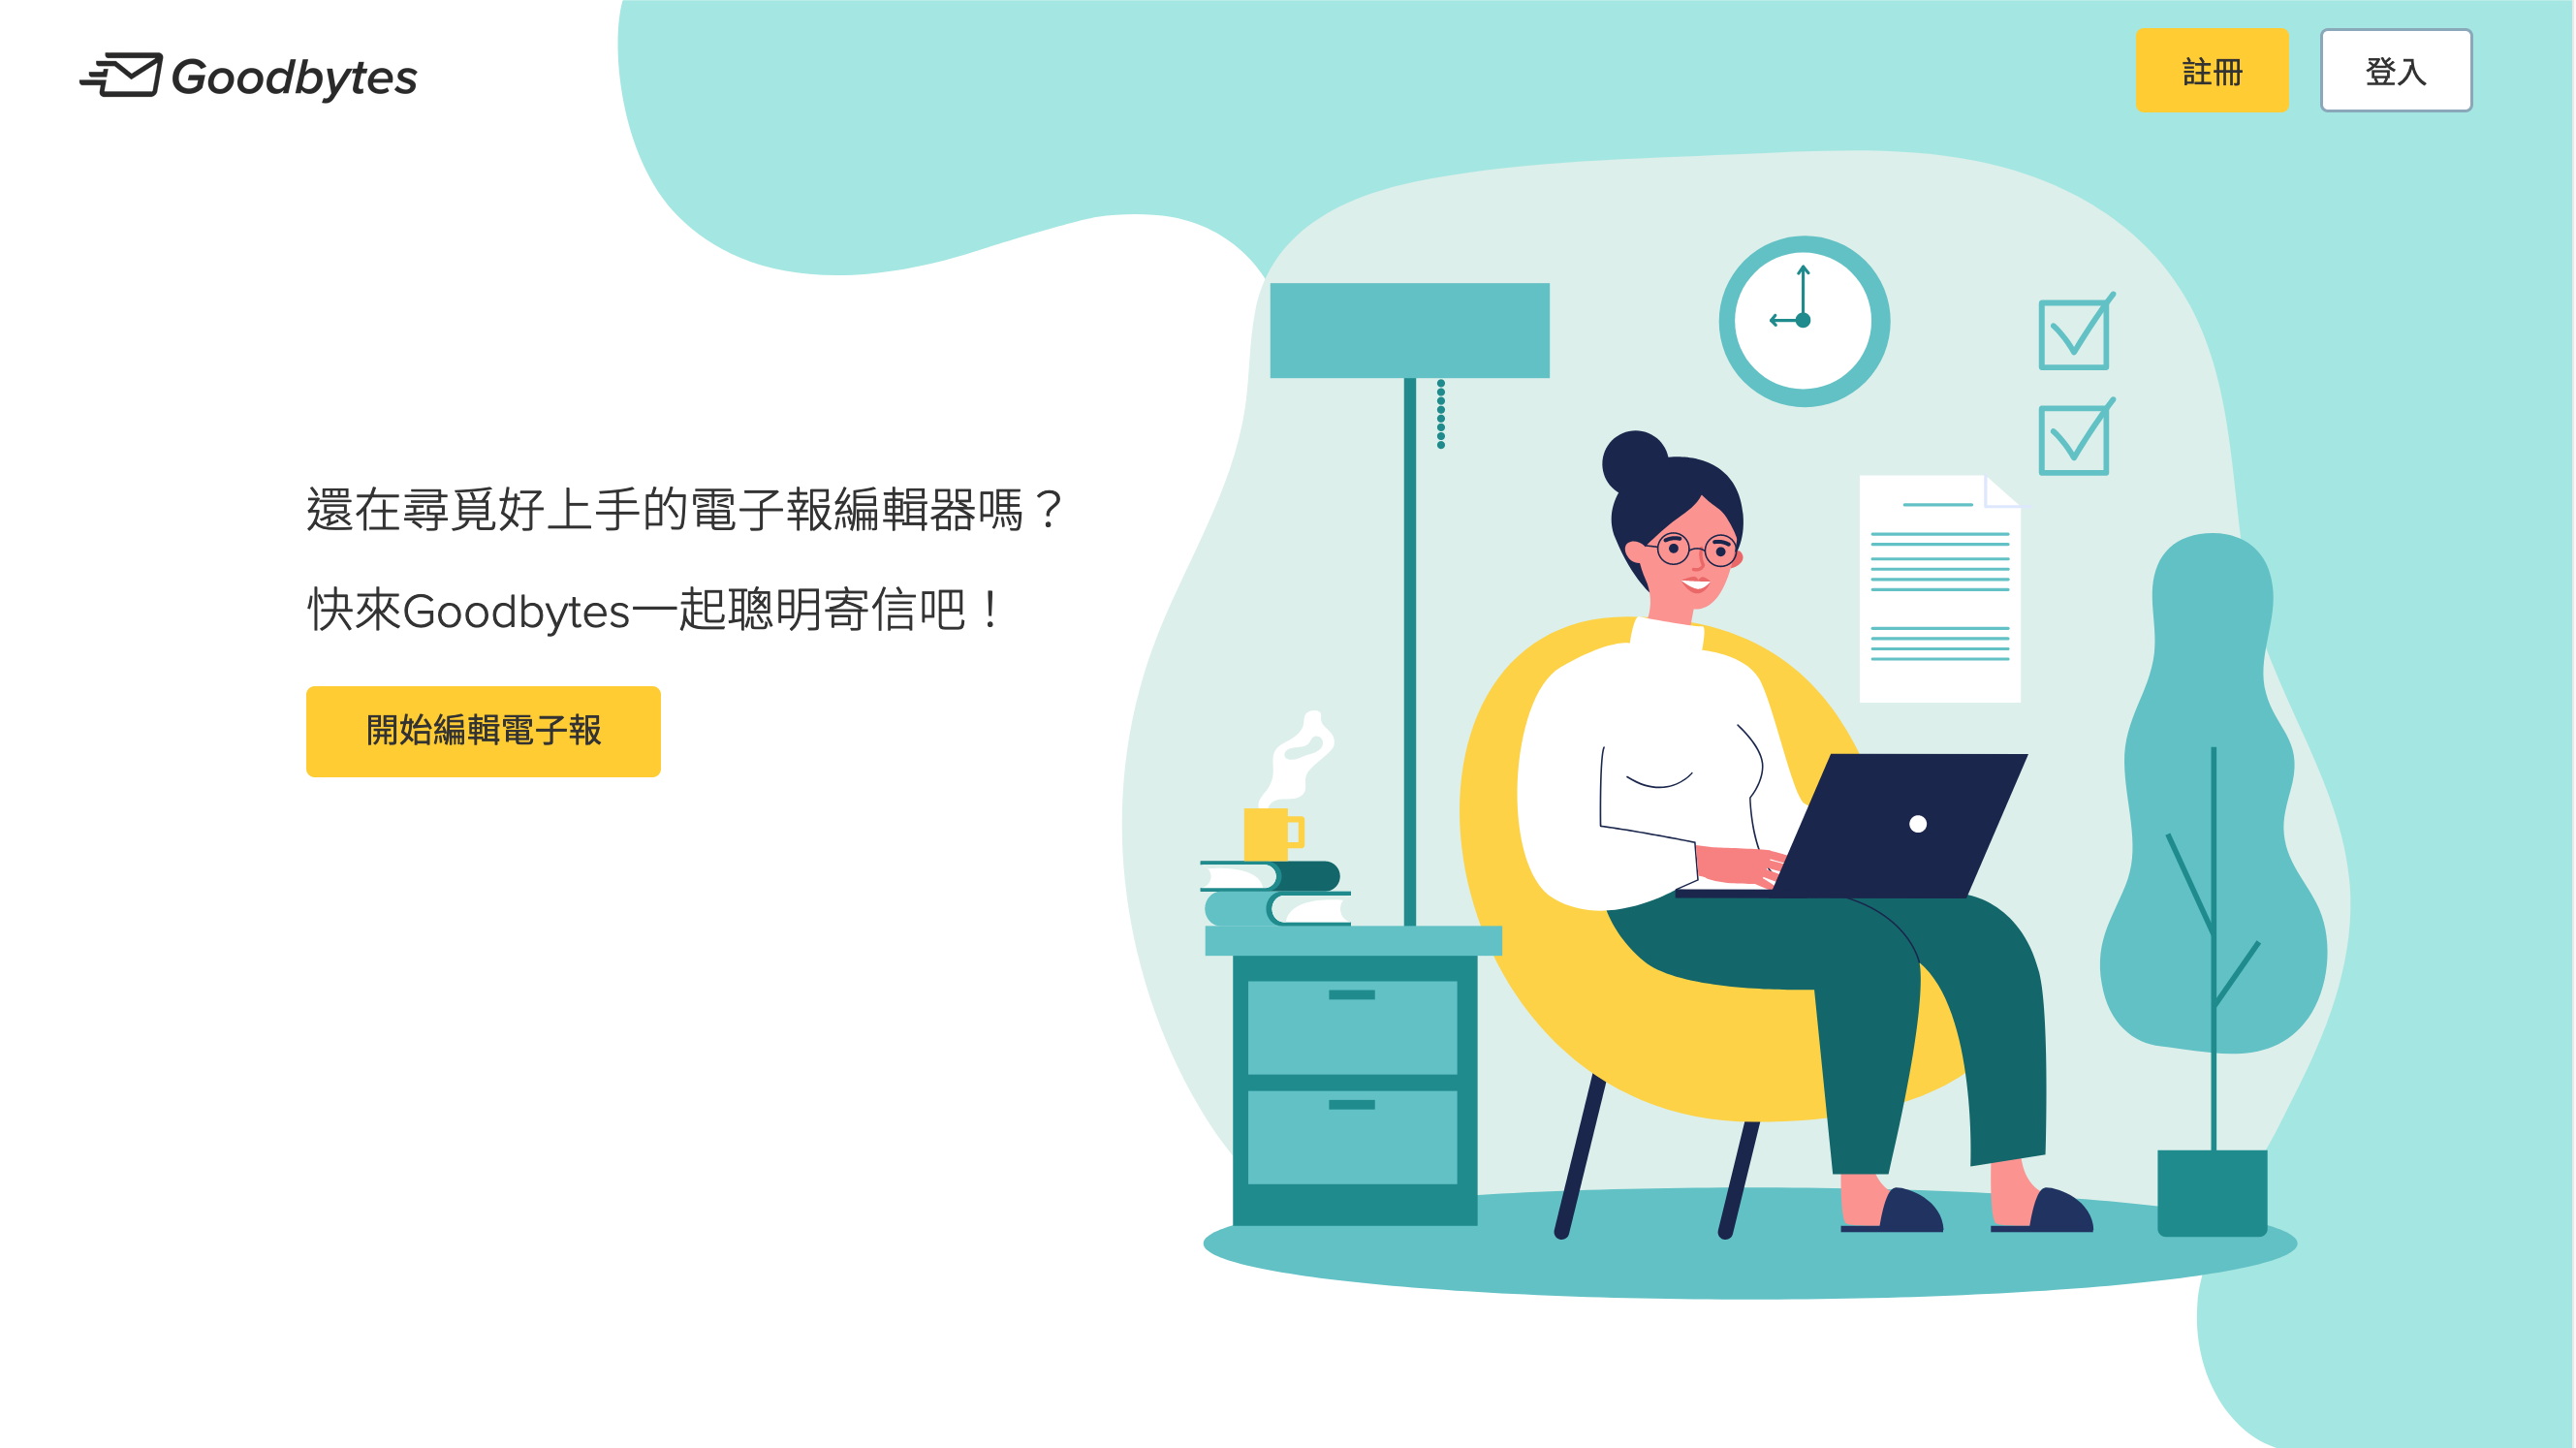
\includegraphics[width=7cm]{shared/landing.png}
\end{center}
\end{minipage}
\section{工作經歷}
\setlength{\leftskip}{1em} 
\begin{cvtable*}

  \hspace*{-.5em}\entry{寶成工業} & 2015/07--2019/10 \\[1em]

  \entry{SAP專案導入& 內部講師} & 臺灣臺中 \\
\begin{itemize}
    \item 分析胡志明指定工廠轄下12個品牌生產數據,協助工廠6個月內成功轉換SAP資料邏輯
    \item 4個月內協助工廠建立3組SAP專責維運團隊,包含臺籍、陸籍、越籍共120人 
\end{itemize}
& 2019/06--2019/10 \\

\entry{運動鞋開發報價,課長} & 越南胡志明 \\
\begin{itemize}
\item 協助Salomon, Arc'teryx, Mavic與Wilson四大品牌下單客戶關係維護
\item 負責上述運動品牌每年600萬雙、 1億2千萬美金營業額之產品報價
\item 每半年提出一份基於生產數據分析之商業簡報予客戶,以協議雙方來年生意版圖 
\item 管理臺籍、越籍10人小隊
\end{itemize} & 2017/05--2019/05 \\

\end{cvtable*}

\begin{cvtable*}
\entry{運動鞋開發報價,管理師} & 中國東莞 \\
\begin{itemize}
\item 審閱與簽署每季上百份供應鏈報價單
\item 獨立負責個別產品生產、原料耗用之成本分析表 
  
\end{itemize}  & 2015/07--2017/04 \\

\entry{花旗商業銀行} & 臺灣臺北 \\
\begin{itemize}
\item 信用卡資料審核
\end{itemize} & 2013/07--2014/11 \\

\end{cvtable*}
\setlength{\leftskip}{0pt} 

\section{\bfseries 教育背景}
\begin{cvtable*}

  \hspace*{-.5em}\entry{Astro Camp 五倍紅寶石} & 臺灣臺北 \\
  HTML, CSS, JavaScript, Ruby, Rails & 2020/03- 2020/06 \\
  \tablespacer

  \hspace*{-.5em}\entry{國立東華大學, 人文社會科學院} & 臺灣花蓮  \\
  經濟/ 財金雙學士  & 2013/06 畢業  \\
  \tablespacer
\end{cvtable*}

\section{\bfseries 技能}
\begin{cvtable*}
  \begin{itemize}
    \item{語言:中文(母語), 英文(流利/ TOEIC 840),越文(A2)}
    \item Microsoft Excel樞紐分析, Google Docs, iWork
    \item 專案時程管理, 經驗4年
    \item 團隊激勵與管理,經驗2年
  \end{itemize}

\end{cvtable*}

\end{document}
